
Um aus den Bilddaten, die während Feldversuchen gesammelt werden, sinnvolle Erkenntnisse zu gewinnen, ist es entscheidend, die Daten effektiv zu strukturieren. Dies erleichtert die effiziente Speicherung und ermöglicht leistungsstarke Datenabfragefunktionen, wie z. B. das patter matching, die für eine umfassende Analyse wichtig sind. Hierfür ist der Einsatz eines Datenbanksystems sinnvoll.

Die im Feld gesammelten Daten werden zunächst in der Datenbank gespeichert und zu einem späteren Zeitpunkt analysiert.

Im Folgenden werden die Schritte zur Auslegung der Datenbank dargestellt. Der Code ist in Section \ref{sect:code}

\subsubsection{Anforderungsanalyse}

Die Anforderungen ergeben sich aus der Funktionsweise des Messaufbaus.

Die Datenbank in dieser Bachelorarbeit wird relativ klein sein, da die Feldversuche zeitintensiv sind. Es wird vermutet, dass maximal 1000 Messungen mit jeweils 3 Taps und je 100 Kreisen durchgeführt werden.

Die Datenbank ist grösser angelegt, als sie für die Vorversuche in der Bachelorarbeit benötigt wird.

Es gibt vier Benutzer die mit der Datenbank interagieren. In der Grafik \ref{fig:user-db-entwurf} sind die schematische Darstellung.

\begin{figure}
    \centering
    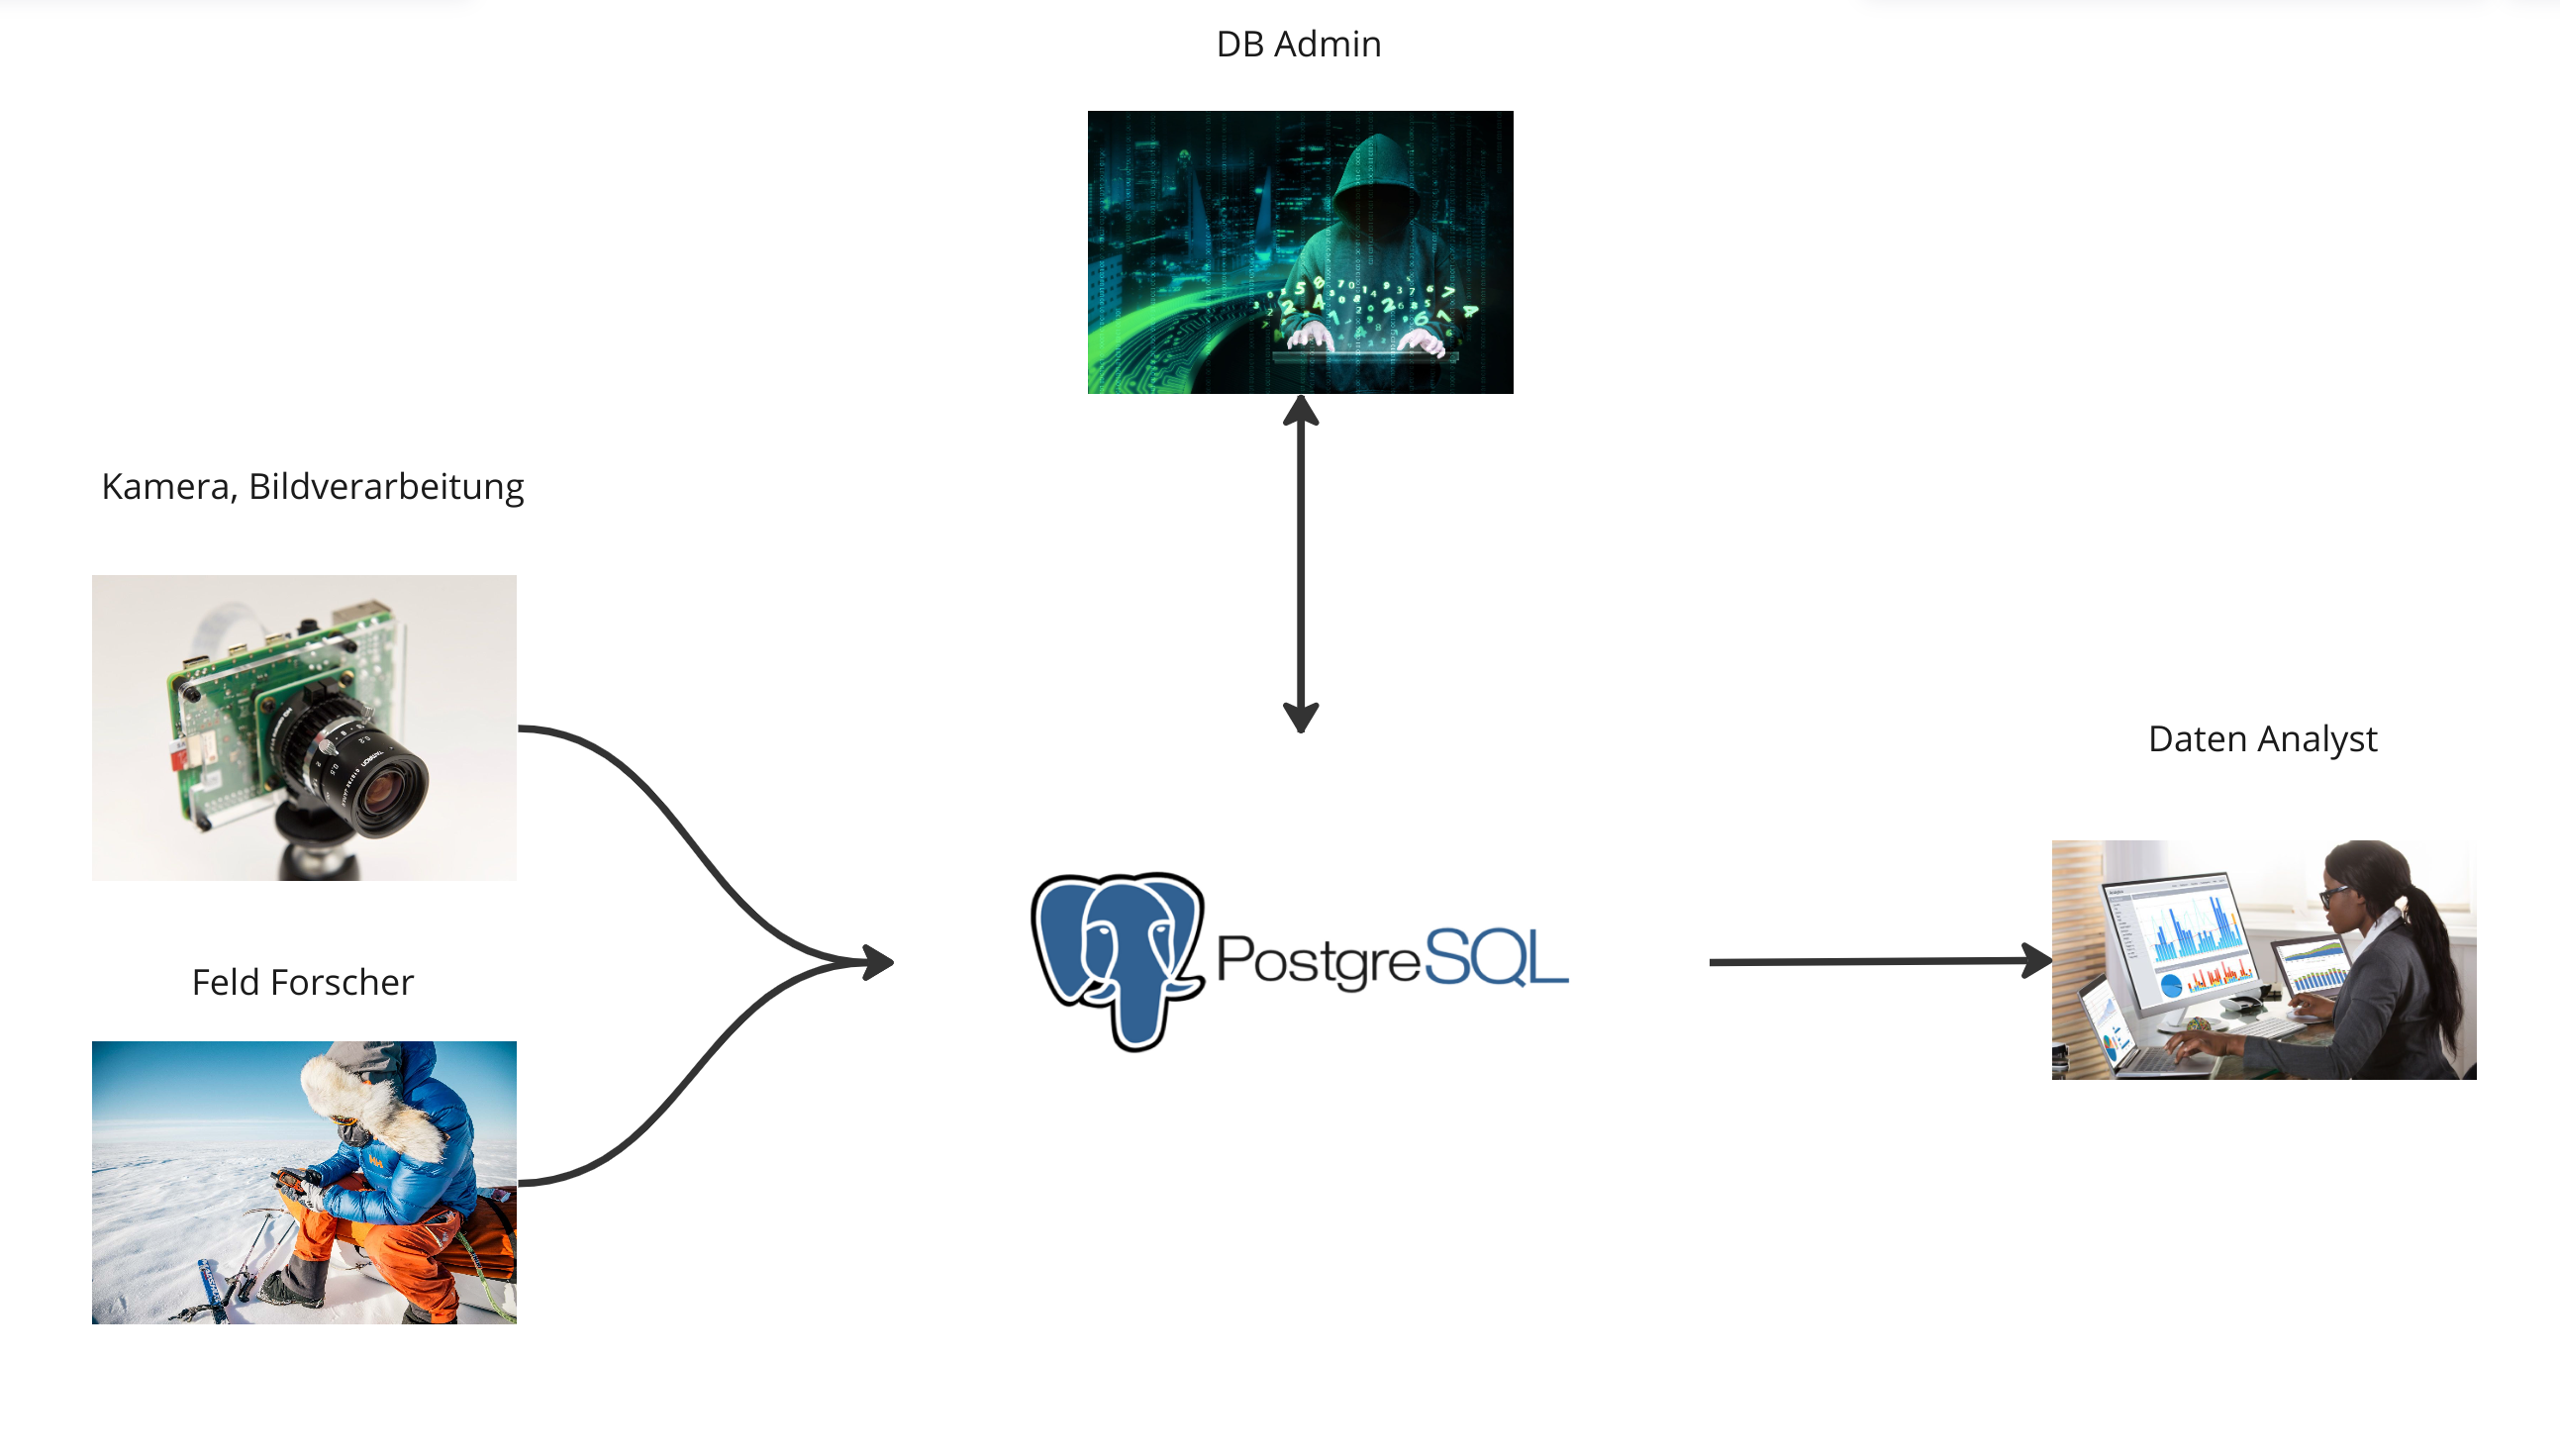
\includegraphics[width=0.8\textwidth]{Bilder/Screenshotfrom2024-04-0115-26-08.png}
    \caption{Benutzer der Datenbank}
    \label{fig:user-db-entwurf}
\end{figure}

\begin{enumerate}
\item Die beiden angemeldeten Endbenutzer: Die Kamera, die die Bilder der Taps macht und auswertet, muss die Auswertungen in die Datenbank schreiben.
  \item Der Versuchsdurchführende gibt zusätzliche Informationen über den Versuch an, die er ebenfalls in die Datenbank schreiben muss.
    
    \item Der Analyst wird die Daten abfragen und hoffentlich Informationen daraus gewinnen.
    
    \item Der Datenbankadministrator wird im Normalbetrieb nicht benötigt, sollte jedoch berücksichtigt werden.
\end{enumerate}

Die Anforderungen an die Datenbank und ihre Benutzer werden entsprechend den Anforderungen des Messaufbaus und den Bedürfnissen der Benutzer festgelegt.

\ref{code:User}

\subsubsection{Konzeptueller DB Entwurf}

Mit der Unified Modeling Language (UML) wird die Struktur der Datenbank dargestellt. Diese Darstellung ist noch lösungsunabhängig.

\begin{figure}
    \centering
    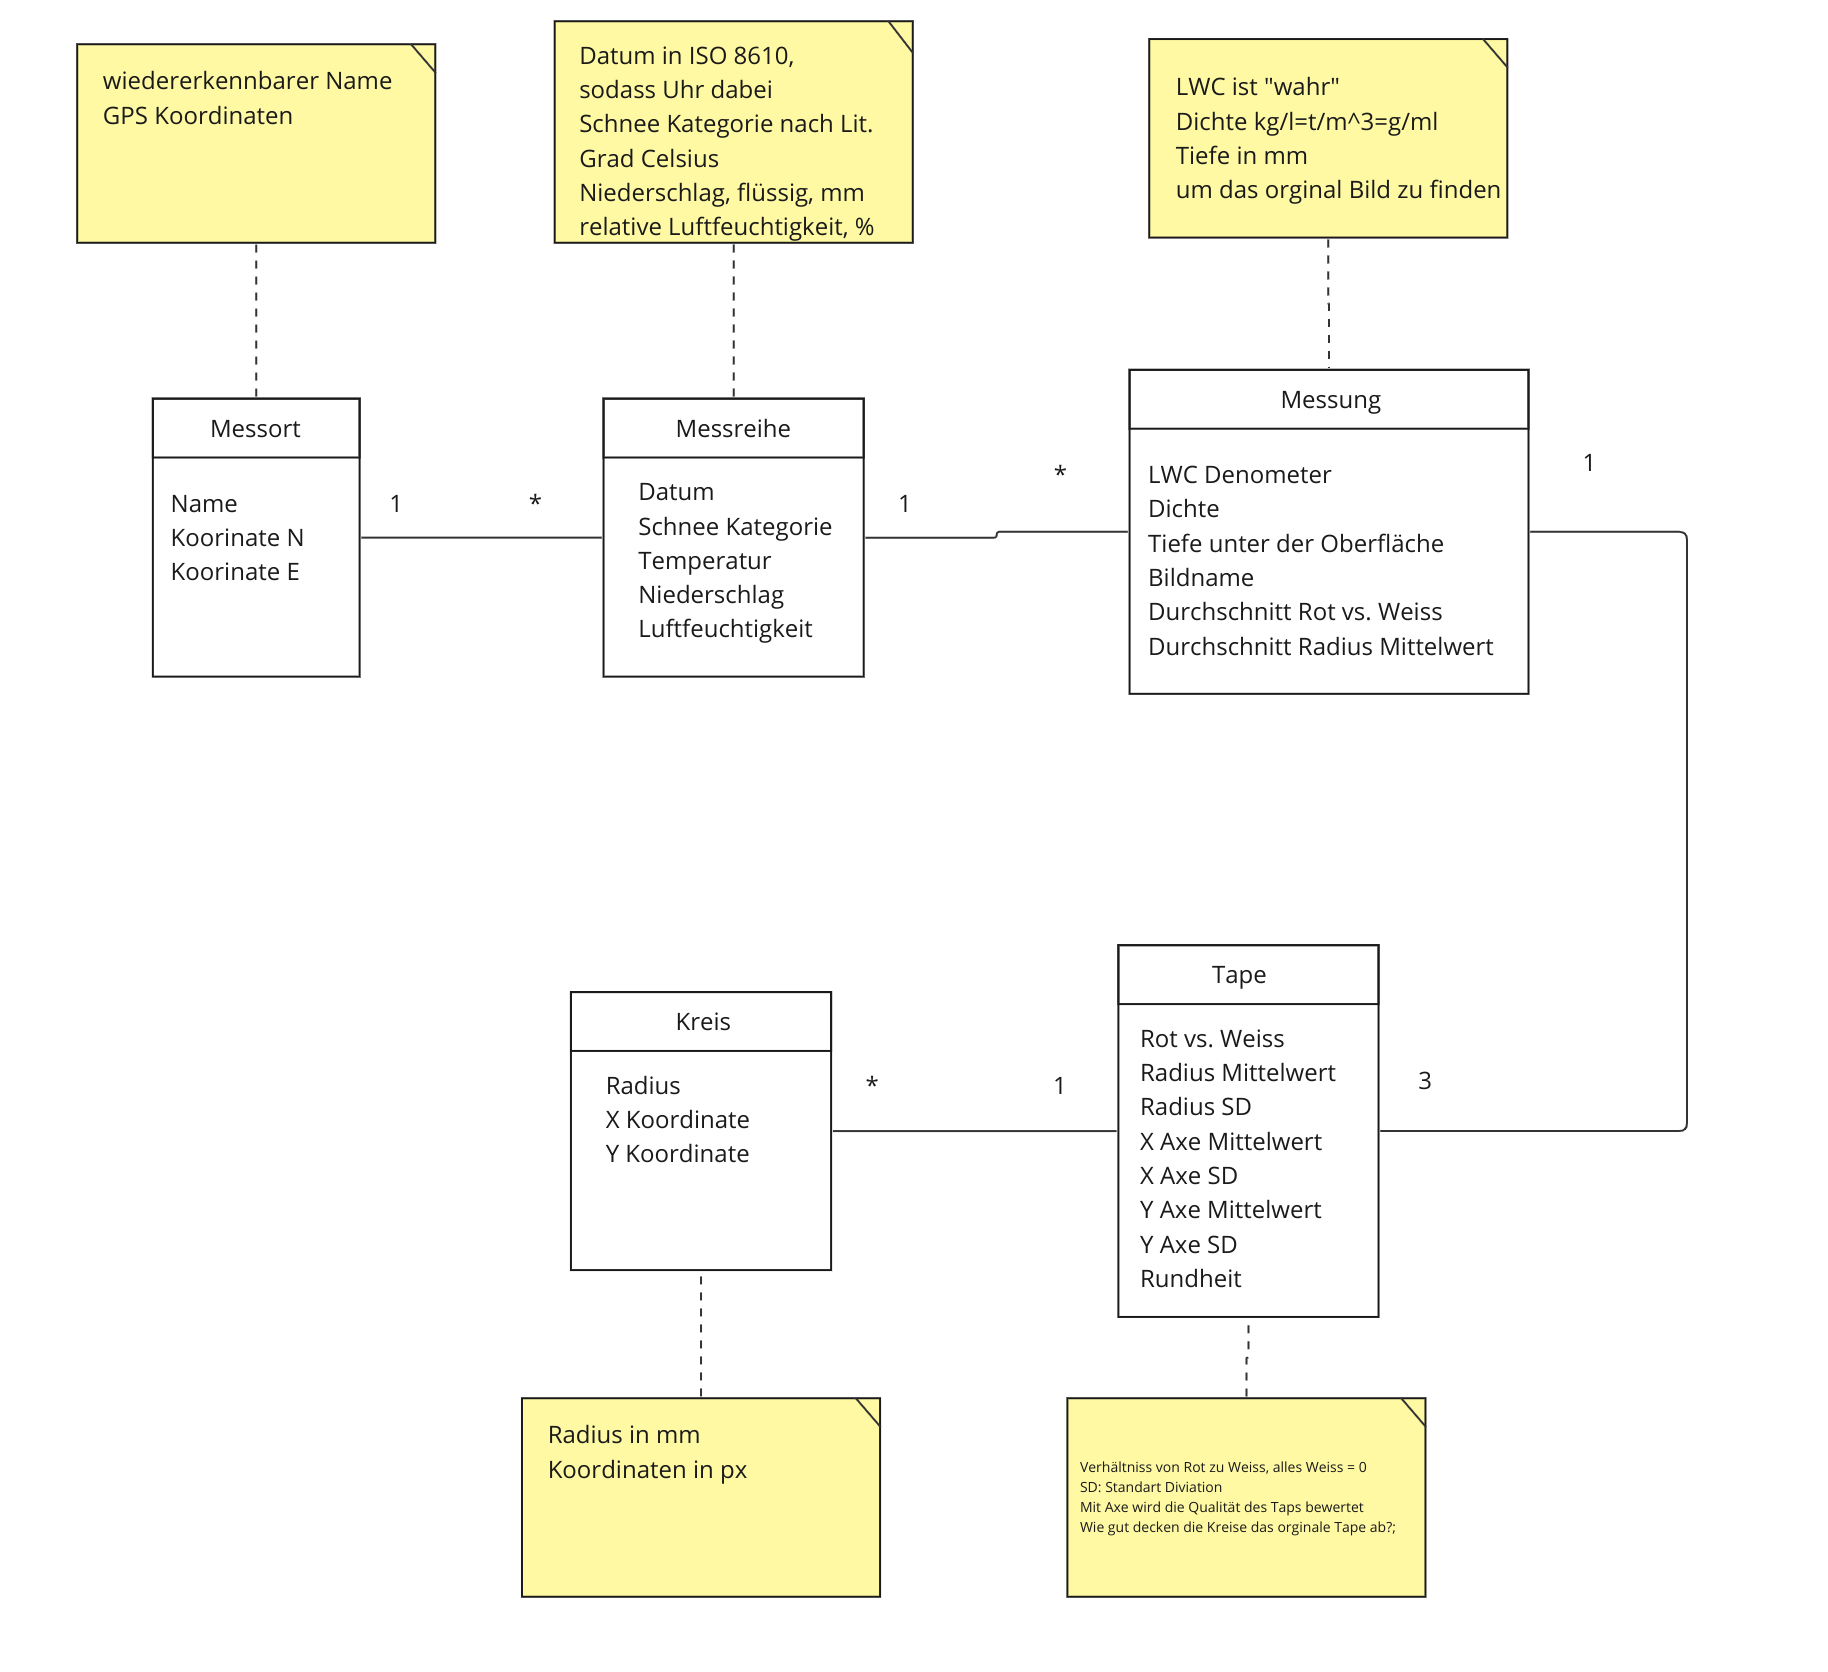
\includegraphics[width=0.8\textwidth]{Bilder/Screenshotfrom2024-04-0113-01-07.png}
    \caption{UML-Diagramm des konzeptuellen DB-Entwurfs}
    \label{fig:uml-db-entwurf}
\end{figure}



\subsubsection{Logischer DB Entwurf}

Um die Datenbank zu implementieren, wurde PostgreSQL gewählt. Es ist ein Free und Open-Source-System, das neue Features wie zum Beispiel JSON-Datentypen unterstützt.

Der folgende SQL-Code initialisiert die Datenbank: \ref{code:DBIni}

\subsubsection{Ansichten für den Analysten}
Das Endziel besteht darin, eine Regression aus den Messungen und Taps zu erstellen, um den 'LWC Denoth' zu bestimmen. Für diese Aufgabe sind nur bestimmte Angaben aus der Datenbank erforderlich.

Hier werden zwei Ansichten erstellt: Der erste ist ein minimalistischer Ansatz, mit dem direkt weitergearbeitet werden kann. Die zweite Ansicht dient dazu, genauer zu verstehen, was in der ersten Ansicht dargestellt ist.

Da die Ansichten für den read only Analysten bestimmt sind, muss keine aktualisierbare Ansicht verwendet werden.

\ref{code:ViewDB}

\subsubsection{Physischer Entwurf}
Für die Beispieldaten wurden Daten aus der Vorstudie \ref{} für eine Messung verwendet.

Die Datenbank wird anfangs viele NULL-Werte enthalten, da beispielsweise die Wetterdaten nicht von einer API gefüllt werden. Das ist auch in Ordnung, da die fehlenden Werte mit 0 aufgefüllt werden.

Die Transaktionen sind in dieser Anwendung unproblematisch, da der Benutzer, der die Inserts durchführt (Raspberry, Feldforscher), zu einem früheren Zeitpunkt arbeitet als der Analyst.

Falls die Datenbank von meinem Laptop auf einen Server ausgelagert wird, werden die folgenden Tools zur Sicherheitsprüfung verwendet: \href{https://www.owasp.org}{www.owasp.org} und \href{http://sqlmap.org/}{http://sqlmap.org/}.

\subsubsection{Python-Interaktion mit der Datenbank}

Für die Interaktion mit der Datenbank werden verschiedene Python-Skripte verwendet, die je nach Benutzer unterschiedliche Aufgaben erfüllen.

Das folgende Python-Skript ist dazu da Bilder von Taps zu analysieren und die daraus gewonnenen Daten in die Datenbank einzufügen. \ref{code:RaspKam}

Das nächste Python-Skript wird interaktiv vom Versuchsleiter verwendet. Zur Zeit ruft das Skript die Bildanalyse auf. \ref{code:FeldUser}


\subsubsection{Nächste Schritte}

Die Python-Programme sollten weiterentwickelt werden, um sämtliche verfügbaren Daten in der Datenbank zu nutzen und um die Funktionalität zu verbessern.

Aktuell läuft die Datenbank mit dem Benutzer "Postgres" auf einem Laptop. Eine Auslagerung auf einen Server ist derzeit keine Priorität, da dies mit Sicherheitsrisiken verbunden ist. Das Hauptziel dieser Produktentwicklungs Bachelorarbeit besteht darin, das Verhalten des Taps zu verstehen. Sobald dieses Ziel erreicht ist, können weitere Schritte zur Optimierung und Sicherung der Datenbankinfrastruktur unternommen werden.

\subsubsection{Code}
\label{sect:code}

\lstinputlisting[language=SQL, basicstyle=\ttfamily\footnotesize, caption={SQL-Code für die Benutzerinitialisierung}, label={code:User}]{UserInizialise.sql}

Die pseudozufällige Passworder sind nicht optimal, besser wäre $SELECT gen_random_uuid();$


\lstinputlisting[language=SQL, basicstyle=\ttfamily\footnotesize, caption={SQL-Code für die DBinitialisierung}, label={code:DBIni}]{DBInizialise.sql}

\lstinputlisting[language=SQL, basicstyle=\ttfamily\footnotesize, caption={SQL-Code für die Views}, label={code:ViewDB}]{ViewsDB.sql}

\lstinputlisting[language=SQL, basicstyle=\ttfamily\footnotesize, caption={SQL-Code für Beispiel Daten}, label={code:ExamData}]{IsertSomeData.sql}

\lstinputlisting[language=Python, basicstyle=\ttfamily\small, caption={Bilderkennung und verarbeitung}, label={code:RaspKam}]{imageToCircle3.py}

\lstinputlisting[language=Python, basicstyle=\ttfamily\small, caption={Bilderkennung und verarbeitung}, label={code:FeldUser}]{splitUpImage.py}
